%
\section{Additional Proofs and Incorporating Item Costs}
 \label{sec:proofs}
%
In this appendix we provide all of the proofs omitted from the main text.
For the results of \secref{sec:greedy}, 
we do so by first explaining how our results generalize to the case where items have costs, and then proving generalizations which incorporate item costs.

\subsection{Incorporating Costs: Preliminaries} \label{sec:incorporating-costs}  

In this section we provide the preliminaries required to define and analyze the versions of our problems with non-uniform item costs.
We suppose each item $\elem\in\groundset$ has a 
cost $c(\elem)$, and the cost of a set
$S\subseteq\groundset$ is given by the modular function $c(S)=\sum_{\elem\in S}c(\elem)$.  
We define the generalizations of problems~(\ref{eq:stochmax}), (\ref{eq:stochcover}), and (\ref{eq:minsumcover}) in \secref{sec:proofs-max-cover},~\secref{sec:proofs-min-cost-cover}, and \secref{sec:proofs-min-sum-cover},  respectively.


Our results are with respect to the greedy policy $\greedypolicy$ and $\alpha$-approximate greedy policies.  With costs, the greedy policy 
selects an item maximizing $\diff{\prlz}{e}/c(e)$, where $\prlz$ is the current partial realization.

\begin{definition}[Approximate Greedy Policy with Costs]
A policy $\policy$ is an $\alpha$-\emph{approximate greedy policy} if 
for all $\prlz$ such that there exists $e \in \groundset$ with $\diff{\prlz}{e} > 0$,
$$\policy(\prlz) \in \set{e \ : \ \frac{\diff{\prlz}{e}}{c(e)} \ \ge
  \ \frac{1}{\alpha} \max_{e'} \paren{\frac{\diff{\prlz}{e'}}{c(e')} }
},$$ 
and $\policy$ terminates upon observing any $\prlz$ such that $\diff{\prlz}{e} \le 0$ for all $e \in
\groundset$.
That is, an $\alpha$-approximate greedy policy always obtains at least 
$(1/\alpha)$ of the maximum possible ratio of conditional expected
marginal benefit to cost, and terminates when no more benefit can be
obtained in expectation.
A \emph{greedy policy} is any $1$-approximate greedy policy.
\end{definition}


It will be convenient to imagine the policy executing over time, such that 
when a policy $\policy$ selects an item $e$, it starts to \emph{run} $e$, and \emph{finishes running} $e$ after  
$c(e)$ units of time.
We next generalize the definition of policy truncation.  Actually we require three such generalizations, which are all equivalent in the unit cost case.
%
%

\begin{definition}[Strict Policy Truncation] \label{def:strict-prune}
The \emph{strict level $t$ truncation} of a policy $\policy$, denoted by
$\strictprune{\policy}{t}$, is obtained by running $\policy$ for $t$ time units, and 
unselecting items whose runs have not finished by time $t$.
%
Formally, $\strictprune{\policy}{t}$ has domain 
$\set{\prlz \in \dom(\policy) \ : \ c(\policy(\prlz)) + \sum_{e \in \dom(\prlz)} c(e) \le t}$, 
and agrees with $\policy$ everywhere in its domain.
\end{definition}


\begin{definition}[Lax Policy Truncation] \label{def:lax-prune}
The \emph{lax level $t$ truncation} of a policy $\policy$, denoted by
$\laxprune{\policy}{t}$, is obtained by running $\policy$ for $t$ time units, and 
selecting the items running at time $t$.
Formally, $\laxprune{\policy}{t}$ has domain 
$\set{\prlz \in \dom(\policy) \ : \ \sum_{e \in \dom(\prlz)} c(e) < t}$, 
and agrees with $\policy$ everywhere in its domain.
\end{definition}


\begin{definition}[Policy Truncation with Costs] \label{def:policy-truncation-with-costs}
  The \emph{level-$t$-truncation} of a policy $\policy$, denoted by
  $\prune{\policy}{t}$, is a randomized policy obtained by
  running $\policy$ for $t$ time units, and 
  if some item $e$ has been running for $0 \le \tau < c(e)$ time at time $t$, 
  selecting $e$ independently with probability $\tau/c(e)$.
  Formally, $\prune{\policy}{t}$ is a randomized policy that agrees with $\policy$
  everywhere in its domain, has 
  $\dom(\strictprune{\policy}{t}) \subseteq \dom(\prune{\policy}{t}) \subseteq \dom(\laxprune{\policy}{t})$ with certainty,  and  includes each $\prlz \in \dom(\laxprune{\policy}{t}) \setminus \dom(\strictprune{\policy}{t})$
 in its domain 
%
independently with probability $\paren{t - \sum_{e \in \dom(\prlz)} c(e)}/c(\policy(\prlz))$.
\end{definition}

In the proofs that follow, we will need a notion of the conditional
expected cost of a policy, as well as an alternate characterization of
\term monotonicity, based on a notion of policy concatenation.
We prove the equivalence of our two \term monotonicity conditions in~\lemref{lem:monotonicity-equivalence}.

\begin{definition}[Conditional Policy Cost]
%
 %
%
The \emph{conditional policy cost} of $\policy$ conditioned on
$\prlz$, denoted $\condcost{\prlz}{\policy}$, is the expected cost of
the items $\policy$ selects under $\rlzmass{\rlz \mid \prlz}$.  That is, 
$\condcost{\prlz}{\policy} := \expctoverrlz{\rvrlz}{c(\played{\policy}{\rvrlz})  \ \mid \ \rvrlz \sim
  \prlz}$.
%
\end{definition}



\begin{definition}[Policy Concatenation] \label{def:policy-concatenation}
Given two policies $\policy_1$ and $\policy_2$ 
%
define $\append{\policy_1}{\policy_2}$ as the policy obtained by running $\policy_1$ to completion, and then running policy  $\policy_2$ as if from a fresh start, ignoring the information
 gathered\footnote{Technically, if under any realization $\rlz$ policy
   $\policy_2$ selects an item that
   $\policy_1$ previously selected, then $\append{\policy_1}{\policy_2}$
   cannot be written as a function from a set of partial realizations
   to $\groundset$, i.e., it is not a policy.  This can be amended by
   allowing partial realizations to be multisets over elements of
   $\groundset \times \outcomes$, so that, e.g., if $e$ is played
   twice
   then $(e, \prlz(e))$ appears twice in
   $\prlz$.  However, in the interest of readability we will avoid this more cumbersome multiset
   formalism, and abuse notation slightly by calling
   $\append{\policy_1}{\policy_2}$ a policy.  This issue arises
   whenever we run some policy and then run another from a fresh start.}
 during the running of $\policy_1$.
\end{definition}

\begin{definition}[\Term Monotonicity (Alternate Version)] \label{def:monotonicity-append}
A function $f:2^{\groundset} \times O^{\groundset} \to \NonNegativeReals$
is \emph{\term monotone} with respect to distribution $\rlzprior$ 
if for all policies $\policy$ and $\policy'$, 
 it holds that 
$\avgf(\policy)\leq \avgf( \append{\policy'}{\policy})$, where 
$\avgf(\policy) := \expctoverrlz{\rvrlz}{f(\played{\policy}{\rvrlz}, \rvrlz)}$
is defined w.r.t.~$\rlzprior$. 
\end{definition}


\begin{lemma}[\Term Monotonicity Equivalence] \label{lem:monotonicity-equivalence}
Fix a function $f:2^{\groundset} \times O^{\groundset} \to \NonNegativeReals$.
Then $\diff{\prlz}{\elem} \ge 0$ for all $\prlz$ with $\Pr{\rvrlz \sim \prlz} > 0$ and all $e \in \groundset$
if and only if
for all policies $\policy$ and $\policy'$, 
$\avgf(\policy)\leq \avgf( \append{\policy'}{\policy})$. 
\end{lemma}

\begin{proof}
Fix policies $\policy$ and $\policy'$.
We begin by proving $\avgf( \append{\policy'}{\policy}) = \avgf( \append{\policy}{\policy'})$.  Fix any $\rlz$ and 
note that 
$\played{\append{\policy'}{\policy}}{\rlz} = \played{\policy'}{\rlz} \cup  \played{\policy}{\rlz} = \played{\append{\policy}{\policy'}}{\rlz}$.
Hence $$\avgf(\append{\policy'}{\policy}) = \expctoverrlz{\rvrlz}{f(\played{\append{\policy'}{\policy}}{\rvrlz}, \rvrlz)} =
\expctoverrlz{\rvrlz}{f(\played{\append{\policy}{\policy'}}{\rvrlz}, \rvrlz)} = \avgf(\append{\policy}{\policy'}).$$
Therefore 
$\avgf(\policy)\leq \avgf(\append{\policy'}{\policy})$ holds if and
only if $\avgf(\policy)\leq \avgf( \append{\policy}{\policy'})$.  
%


We first prove the forward direction.
Suppose $\diff{\prlz}{\elem} \ge 0$ for all $\prlz$ and all $e \in \groundset$.
Note the expression $\avgf( \append{\policy}{\policy'}) - \avgf(\policy)$ can be written as a conical combination of (nonnegative) $\diff{\prlz}{\elem}$ terms, i.e., 
for some $\alpha \ge \mathbf{0}$,  $\avgf( \append{\policy}{\policy'}) - \avgf(\policy) = \sum_{\prlz,e} \alpha_{(\prlz,e)}\, \diff{\prlz}{\elem}$. 
Hence $\avgf( \append{\policy}{\policy'}) - \avgf(\policy) \ge 0$ and so $\avgf(\policy)\leq \avgf(\append{\policy}{\policy'}) = \avgf(\append{\policy'}{\policy})$.


We next prove the backward direction, in contrapositive form. 
Suppose $\diff{\prlz}{\elem} < 0$ for some $\prlz$ with $\Pr{\rvrlz \sim \prlz} > 0$ and $e \in \groundset$.
Let $e_1, \ldots, e_r$  be the items in $\dom(\prlz)$ and define policies 
$\policy$ and $\policy'$ as follows.  For $i = 1, 2, \ldots, r$, both
$\policy$ and $\policy'$ select $e_i$ and observe $\rvrlz(e_i)$.
If either policy observes $\rvrlz(e_i) \neq \prlz(e_i)$ it immediately terminates, otherwise it continues.
If $\policy$ succeeds in selecting all of $\dom(\prlz)$ then it terminates.
If $\policy'$ succeeds in selecting all of $\dom(\prlz)$ then it selects $e$ and then terminates.
We claim $\avgf( \append{\policy}{\policy'}) - \avgf(\policy) < 0$.
Note that 
%
%
%
$\played{ \append{\policy}{\policy'} }{\rlz} = \played{\policy }{\rlz}$ unless $\rlz \sim \prlz$, and if 
$\rlz \sim \prlz$ then 
$\played{ \append{\policy}{\policy'} }{\rlz} = \played{\policy }{\rlz} \cup \set{e}$ and also 
$\played{\policy }{\rlz}= \dom(\prlz)$.  
Hence 
\begin{eqnarray*}
  \label{eq:1app}
  \avgf( \append{\policy}{\policy'}) - \avgf(\policy) & = & 
 \expctoverrlz{\rvrlz}{f( \played{ \append{\policy}{\policy'} }{\rvrlz}  , \rvrlz) -
   f(  \played{\policy }{\rvrlz}  , \rvrlz)} \\ 
 & = & \expctoverrlz{\rvrlz}{f( \played{ \append{\policy}{\policy'} }{\rvrlz}  , \rvrlz) -
   f( \played{\policy }{\rvrlz}   , \rvrlz) \ | \ \rvrlz\sim\prlz }\cdot  \proboverrlz{\rvrlz}{\rvrlz \sim \prlz}  \\
 & = & \expctoverrlz{\rvrlz}{f(  \dom(\prlz) \cup \set{e}, \rvrlz) -
   f( \dom(\prlz) , \rvrlz) \ | \ \rvrlz\sim\prlz } \cdot \proboverrlz{\rvrlz}{\rvrlz \sim \prlz} \\
 & = & \diff{\prlz}{\elem} \cdot \proboverrlz{\rvrlz}{\rvrlz \sim \prlz}
\end{eqnarray*}
The last term is negative, as $\proboverrlz{\rvrlz}{\rvrlz \sim \prlz} > 0$ and $ \diff{\prlz}{\elem} < 0$ by assumption.
Therefore
$\avgf(\policy) > \avgf( \append{\policy}{\policy'}) = \avgf( \append{\policy'}{\policy})$, which completes the proof.
\ignore{
%
We next prove the backward direction, in contrapositive form. 
Suppose $\avgf(\policy) > \avgf( \append{\policy'}{\policy})$ for some $\policy$ and $\policy'$.
Then $\avgf(\policy) > \avgf( \append{\policy}{\policy'})$ and $\avgf( \append{\policy}{\policy'}) - \avgf(\policy) < 0$.
However, as we mentioned previously $\avgf( \append{\policy}{\policy'}) - \avgf(\policy) $ can be written as a conical combination of $\diff{\prlz}{\elem}$ terms.  Since a conical combination of nonnegative terms is nonnegative, this implies there exist some $\prlz$ and $e$ 
%
such that $\diff{\prlz}{\elem} < 0$.
}
\end{proof}
%
%
%





%
\subsection{Adaptive Data Dependent Bounds with Costs} \label{sec:costs-data-dependent-bounds}  
%

The adaptive data dependent bound has the following generalization with costs.

\begin{lemma}[The Adaptive Data Dependent Bound with Costs] \label{lem:rate-equation-with-costs}
Suppose we have made observations $\prlz$ \mbox{after}
selecting $\dom(\prlz)$.  Let $\policy^*$ be any policy.
Then for \term monotone submodular $f:2^\groundset \times
\outcomes^{\groundset} \to \NonNegativeReals$ 
\begin{equation}
  \label{eq:data-dependent-bound-adaptive-with-costs}
\diff{\prlz}{\policy^*} \ \le \ Z \ \le \  
\condcost{\prlz}{\policy^*} \max_{e} \paren{\frac{\diff{\prlz}{e}}{c(e)}}
%
%
%
\end{equation}
where $Z = \max_w \set{ \sum_{e \in \groundset} w_e \,\diff{\prlz}{e} \ :
  \ \sum_e
  c(e) w_e \le \condcost{\prlz}{\policy^*} \text{ and } \forall e \in \groundset, 0 \le w_e \le 1
}$.  
%
%
%
\end{lemma}

%
%
%

%



\begin{proof} 
%
%
 %
%
Order the items in $\dom(\prlz)$ arbitrarily, and 
consider the policy $\policy$ that for each $e \in \dom(\prlz)$ in
order selects $e$, terminating if $\rvrlz(e) \neq \prlz(e)$ and
proceeding otherwise, and, should it succeed in selecting all of
$\dom(\prlz)$ without terminating (which occurs iff $\rvrlz \sim
\prlz$), then proceeds to run $\policy^*$ as if from a fresh start,
forgetting the observations in $\prlz$.
%
%
%
%
By construction 
the expected marginal benefit of running the $\policy^*$ portion of
$\policy$ conditioned on $\rvrlz \sim \prlz$ equals $\diff{\prlz}{\policy^*}$.
For all $e \in \groundset$, let $w(e) = \Pr{e \in
  \played{\policy}{\rvrlz} \ \mid \ \rvrlz \sim \prlz}$
be the probability that $e$ is selected when running $\policy$, 
conditioned on $\rvrlz \sim \prlz$.
Whenever some $e \in \groundset \setminus \dom(\prlz)$ is selected by $\policy$, the current partial realization
$\prlz'$ contains $\prlz$ as a subrealization; hence \term
submodularity implies $\diff{\prlz'}{e} \le \diff{\prlz}{e}$.
It follows that the total contribution of $e$ to $\diff{\prlz}{\policy^*}$
is upper
bounded by $w(e) \cdot \diff{\prlz}{e}$.
Summing over $e  \in \groundset \setminus \dom(\prlz)$, 
%
we get a bound of 
$\diff{\prlz}{\policy^*} \le \sum_{e  \in \groundset \setminus
     \dom(\prlz)} w(e) \diff{\prlz}{e}$.
Next, note that each $e \in \groundset \setminus
\dom(\prlz)$ contributes $w(e)c(e)$ cost to $\condcost{\prlz}{\policy^*}$.
Hence it must be the case that 
$\sum_{e  \in \groundset \setminus \dom(\prlz)} w(e)c(e) \le \condcost{\prlz}{\policy^*}$.
Obviously, $w(e) \in [0,1]$ for all $e$, since $w(e)$ is a probability.
Hence $\diff{\prlz}{\policy^*} \le \sum_{e  \in \groundset \setminus \dom(\prlz)} w(e)
\diff{\prlz}{e} \le Z$ because setting $w_e = w(e)$ is feasible for the
the linear program for which $Z$ is the optimal value.

%
%
%
%

To show $Z \le \condcost{\prlz}{\policy^*} \max_{e} \paren{\diff{\prlz}{e} /
  c(e)}$, consider any feasible solution $w$ to the linear program
defining $Z$.  It attains objective value 
$$\sum_{e \in \groundset} w_e \,\diff{\prlz}{e} \le \sum_{e \in
  \groundset} w_e c(e) \frac{\diff{\prlz}{e}}{c(e)} \le \sum_{e \in
  \groundset} w_e c(e) \max_{e \in \groundset} \paren{\frac{\diff{\prlz}{e}}{c(e)}} \le
\condcost{\prlz}{\policy^*}  \max_{e \in \groundset} \paren{\frac{\diff{\prlz}{e}}{c(e)}} $$
since $ \sum_{e \in \groundset} w_e c(e) \le \condcost{\prlz}{\policy^*} $ by
the feasibility of $w$.
\end{proof}

A simple greedy algorithm can be used to compute $Z$; we provide
pseudocode for it in~\algref{alg:data-dependent-bound}.
The correctness of this algorithm is more readily discerned upon rewriting
the linear program using variables $x_e = c(e) w_e$ to obtain 
$$Z = \max_x \set{ \sum_{e \in \groundset} x_e \paren{\diff{\prlz}{e}/c(e)} \ :
  \ \sum_e
  x_e \le \condcost{\prlz}{\policy^*}\text{ and } \forall e \in \groundset, 0
  \le x_e \le c(e)}.$$
Intuitively, it is clear that to optimize $x$ we should shift mass
towards variables with the highest $\diff{\prlz}{e}/c(e)$ ratio.
Clearly, any optimal solution has $\sum_e x_e = \condcost{\prlz}{\policy^*}$. 
Moreover, in any optimal solution, 
$\diff{\prlz}{e}/c(e) > \diff{\prlz}{e'}/c(e')$ implies 
$x_e = c(e)$ or $x_{e'} = 0$, 
since otherwise it would be possible to shift mass from $x_{e'}$ to
$x_{e}$ and obtain an increase in objective value.
If the $\diff{\prlz}{e}/c(e)$ values are distinct for distinct items,
there will be a unique solution satisfying these constraints, which 
\algref{alg:data-dependent-bound} will compute.
Otherwise, we imagine perturbing each $\diff{\prlz}{e}$ by 
independent random quantities $\epsilon_e$ drawn uniformly from
$[0,\epsilon]$ to make them distinct.  This changes the optimum value
by at most $|\groundset| \epsilon$, which vanishes as we let $\epsilon $ tend
towards zero.  Hence any solution satisfying $\sum_e x_e = \condcost{\prlz}{\policy^*} $
and $\diff{\prlz}{e}/c(e) > \diff{\prlz}{e'}/c(e')$ implies 
$x_e = c(e)$ or $x_{e'} = 0$ is optimal.
Since \algref{alg:data-dependent-bound} outputs the value of such a
solution, it is correct.
%
%



%
%
%


%
%
%
%

%
%
%
%
%
%
%
%
%
%

\begin{algorithm}
 \KwIn{Groundset $\groundset$; Partial realization $\prlz$; Costs
   $c:\groundset \to \nats$;  Budget $C = \condcost{\prlz}{\policy^*}$;   
   Conditional expected marginal benefits $\diff{\prlz}{e}$ for all $e \in \groundset$.}  
\KwOut{\ignore{Data dependent bound} $Z = \max_w \set{ \sum_{e \in \groundset} w_e \,\diff{\prlz}{e} \ :
  \ \sum_e
  c(e) w_e \le \condcost{\prlz}{\policy^*} \text{ and } \forall e \in \groundset, 0 \le w_e \le 1
}$}
\Begin{
  \mbox{Sort $\groundset$ \ignore{in decreasing order} by
    $\diff{\prlz}{e}/c(e)$, so that $\frac{\diff{\ \prlz}{e_1\ }}{c(e_1)}
  \ge \frac{\diff{\ \prlz}{e_2\ }}{c(e_2)} \ge \ldots \ge
  \frac{\diff{\ \prlz}{e_n\ }}{c(e_n)}$}\;

   Set $w \gets \mathbf{0}$;  $i \gets 0$; $a \gets 0$; $z \gets 0$; $e \gets \NULL$\;
   \While{$a < C$}{
       $i \gets i+1$; \ \  $e \gets e_i$\;  
       $w_e \gets \min \set{1, C - a}$\;
       $a \gets a + c(e) w_e$; \ \
       $z \gets z + w_e \diff{\prlz}{e}$; 
   }
   Output $z$;
 } \label{alg:data-dependent-bound} \caption{Algorithm to compute the
   data dependent bound $Z$ of Lemma~\ref{lem:rate-equation-with-costs}.}
\end{algorithm}

%
\subsection{The Max-Cover Objective} \label{sec:proofs-max-cover}  
%

%

With item costs, the Adaptive Stochastic Maximization problem becomes one of finding some
\begin{equation}
\policy^{*}\in\argmax_{\policy} \avgf(\prune{\policy}{\budget}) 
\label{eq:stochmax-costs}
\end{equation} where $\budget$ is a budget on the cost of selected
items, and we define $\avgf(\policy)$ for a randomized policy
$\policy$ to be 
$\avgf(\policy) := \expct{f(\played{\policy}{\rvrlz}, \rvrlz)}$ as before,
where the expectation is now over both $\rvrlz$ and the internal
randomness of $\policy$ which determines 
$\played{\policy}{\rlz}$ for each $\rlz$.
We prove the following generalization of~\thmref{thm:max-cover}.


\begin{theorem} \label{thm:max-cover-with-costs}
Fix any $\alpha \ge 1$ and item costs $c:\groundset \to \nats$.
If $f$ is \term monotone and \term submodular with respect to the
distribution 
$\rlzprior$, and $\policy$ is an
$\alpha$-approximate greedy policy, then for all policies $\policy^*$ and positive
integers $\ell$ and $k$ 
\[
\avgf(\prune{\policy}{\ell}) > \paren{1 - e^{-\ell/\alpha k}}
\avgf(\prune{\policy^*}{k}) 
\mbox{.}
\]
%
%
%
%
\end{theorem}


\begin{proof}
%
%
The proof goes along the lines of the performance analysis of the
greedy algorithm for maximizing a submodular function subject to
a cardinality constraint of~\citet{nemhauser78}.  An
extension of that analysis to $\alpha$-approximate greedy algorithms, 
which is analogous to ours but for the nonadaptive case, is shown by~\citet{goundan07}.
%
For brevity, we will assume without loss of generality that
 $\policy = \prune{\policy}{\ell}$ and $\policy^* = \prune{\policy^*}{k}$.  
Then for all $i$, $0 \le i < \ell$
\begin{equation}
  \label{eqn:ee1}
  \avgf(\policy^*) \ \ \le \ \ \avgf(
  \append{\prune{\policy}{i}}{\policy^*}) \ \ \le \ \ \avgf(\prune{\policy}{i}) + \alpha k \paren{\avgf(\prune{\policy}{i+1}) - \avgf(\prune{\policy}{i})}. 
\end{equation}
%
%
%
%
%
%
%
%
The first inequality is due to the \term monotonicity of $f$ and~\lemref{lem:monotonicity-equivalence}, from which we
  may infer $\avgf(\policy_2) \le \avgf(\append{\policy_1}{\policy_2})$ for any $\policy_1$ and $\policy_2$.
%
The second inequality may be obtained as 
%
%
a corollary of~\lemref{lem:rate-equation-with-costs} as follows.
Fix any partial realization $\prlz$ of the form 
$\set{(e, \rlz(e)) : e \in \played{\prune{\policy}{i}}{\rlz}}$
for some $\rlz$.
%
%
Consider $\diff{\prlz}{\policy^*}$, which equals 
the expected marginal benefit of the $\policy^*$ portion of
$\append{\prune{\policy}{i}}{\policy^*}$ conditioned on $\rvrlz \sim
\prlz$.  
%
%
%
%
%
\lemref{lem:rate-equation-with-costs} allows us to bound it as
$$\expct{\diff{\prlz}{\policy^*}} \ \le \ \expct{\condcost{\prlz}{\policy^*}} \cdot
\max_{e} \paren{\diff{\prlz}{e}/c(e)},$$ 
where the expectations are taken
over the internal randomness of $\policy^*$, if there is any.  Note
that since $\policy^*$ has the form $\prune{\policy'}{k}$ for some
$\policy'$ we know that for all $\rlz$,
$\expct{c(\played{\policy^*}{\rlz})} \le k$, where the
expectation is again taken over the internal randomness of $\policy^*$.
Hence $\expct{\condcost{\prlz}{\policy^*}} \le k$ for all $\prlz$.  It
follows that $\expct{\diff{\prlz}{\policy^*}} \le k \cdot
\max_{e} \paren{\diff{\prlz}{e}/c(e)}$.
%
By definition of an $\alpha$-approximate greedy policy, $\policy$
obtains at least $(1/\alpha)\max_{e}
\paren{\diff{\prlz}{e}/c(e)} \ge \expct{\diff{\prlz}{\policy^*}} / \alpha k$ 
expected marginal benefit per unit cost 
 in a step immediately following its observation of $\prlz$.
%
%
%
%
Next we take an appropriate convex combination of the previous inequality
with different values of $\prlz$.
%
Let $\rvprlz$ be a random partial realization distributed as 
$\rlzmassover{\rvprlz}{\prlz} := \prob{\rvprlz = \prlz \mid \exists \rlz.\ \prlz = \set{(e, \rlz(e)) : e \in \played{\prune{\policy}{i}}{\rlz}}}$
%
%
Then 
%
\begin{eqnarray*}
  \avgf(\prune{\policy}{i+1}) -  \avgf(\prune{\policy}{i}) & \ge & \expct{ \frac{1}{\alpha}\,\max_{e}
\paren{\frac{\diff{\rvprlz}{e}}{c(e)}} } \\
 &  \ge & \expct{
\frac{\expct{\diff{\rvprlz}{\policy^*}}}{\alpha k} }\\
  & = & \frac{ \avgf(
    \append{\prune{\policy}{i}}{\policy^*})  -
    \avgf(\prune{\policy}{i})} {\alpha k} 
\end{eqnarray*}
%
%
%
%
%
%
%
%
%
%
%
%
%
%
%
\noindent
A simple rearrangement of terms then yields the second inequality in~(\ref{eqn:ee1}).

%
%
%
%
%
%
%




Now define $\Delta_i := \avgf(\policy^*) - \avgf(\prune{\policy}{i})$,
so that~(\ref{eqn:ee1}) implies $\Delta_i \le \alpha k(\Delta_i
  - \Delta_{i+1})$, from which we infer
  $\Delta_{i+1} \le \paren{1-\frac{1}{\alpha k}}\Delta_{i}$ and hence 
$\Delta_{\ell} \le \paren{1 - \frac{1}{\alpha k}}^{\ell} \Delta_0 <
e^{-\ell/\alpha k} \Delta_0$, where for this last inequality we have used
the fact that $1 - x < e^{-x}$ for all
$x > 0$.
Thus 
$\avgf(\policy^*) - \avgf(\prune{\policy}{\ell}) < e^{-\ell/\alpha k} \paren{\avgf(\policy^*) -
  \avgf(\prune{\policy}{0})} \le e^{-\ell/\alpha k} \avgf(\policy^*)$ so
$\avgf(\policy) > (1-e^{-\ell/\alpha k})\avgf(\policy^*)$.

\ignore{
Let $T = \prune{T^{\policy}}{\ell}, T^* = \prune{T^{\policy^*}}{k}$.  
Then for all $i$, $0 \le i < \ell$
\begin{eqnarray}%
\avgf(T^*) & \le & \avgf( \append{\prune{T}{i}}{T^*}) \\[-1mm]
  & = &  \avgf(\prune{T}{i}) + \sum_{j=1}^{k} 
          \paren{ \avgf(\append{\prune{T}{i}}{\prune{T^*}{j}}) -
                  \avgf(\append{\prune{T}{i}}{\prune{T^*}{j-1}})   } \\[-1mm]
  & \le & \avgf(\prune{T}{i}) +  \sum_{j=1}^{k} 
          \expct{\avgf\paren{\treeSmush{(\append{\prune{T}{i}}{T^*})}{i}{i+j}
  }  - \avgf(\prune{T}{i})  } \label{eqn:e3}\\[-1mm]
 & \le &  \avgf(\prune{T}{i}) + \alpha \sum_{j=1}^{k} 
          \paren{\avgf(\prune{T}{i+1}) - \avgf(\prune{T}{i})} \label{eqn:e4}
  \end{eqnarray}        
The first inequality is due to the \term monotonicity of $f$, from which we
  may infer $\avgf(T_2) \le \avgf(\append{T_1}{T_2})$ for any $T_1$ and $T_2$.
The second is a simple telescoping sum.  The third is a direct
  application of the \term submodularity guarantee of $f$ with $\append{\prune{T}{i}}{\prune{T^*}{j}}$ at levels $i$ and $i+j$, 
 and the fourth is by the
  definition of an $\alpha$-approximate greedy policy.
Now define $\Delta_i := \avgf(T^*) - \avgf(\prune{T}{i})$, so that~\eqnref{eqn:e4} implies $\Delta_i \le \alpha k(\Delta_i
  - \Delta_{i+1})$, from which we infer
  $\Delta_{i+1} \le \paren{1-\frac{1}{\alpha k}}\Delta_{i}$ and hence 
$\Delta_{\ell} \le \paren{1 - \frac{1}{\alpha k}}^{\ell} \Delta_0 <
e^{-\ell/\alpha k} \Delta_0$, where for this last inequality we have used
the fact that $1 - x < e^{-x}$ for all
$x > 0$.
Thus 
$\avgf(T^*) - \avgf(\prune{T}{\ell}) < e^{-\ell/\alpha k} \paren{\avgf(T^*) -
  \avgf(\prune{T}{0})} \le e^{-\ell/\alpha k} \avgf(T^*)$ so
$\avgf(T) > (1-e^{-\ell/\alpha k})\avgf(T^*)$.
} %
\end{proof}



%
\subsection{The Min-Cost-Cover Objective} \label{sec:proofs-min-cost-cover}  
%

In this section, we provide arbitrary item cost generalizations
of~\thmref{thm:min-set-cover-avg-generalized} and
\thmref{thm:min-set-cover-wc-generalized}. 
With item costs the Adaptive Stochastic Minimum Cost Cover problem
becomes one of finding, for some quota on utility $\quota$,   
\begin{equation}
\policy^{*}\in\argmin_{\policy} \acst{\policy}\text{ such that }
f(\played{\policy}{\rlz},\rlz)\geq \quota\text{ for all
}\rlz,\label{eq:stochcover-with-costs}
\end{equation}
where  $\acst{\policy}:=\expctoverrlz{\rlz}{c(\played{\policy}{\rvrlz})}$.
Without loss of generality, we may take a truncated version of $f$,
namely $(A, \rlz) \mapsto \min \set{\quota, f(A, \rlz)}$, and
rephrase Problem~(\ref{eq:stochcover-with-costs}) as finding
\begin{equation}
  \label{eq:stochcover-with-costs-coverage}
  \policy^{*}\in\argmin_{\policy} \acst{\policy}\text{ such that }
\policy \text{ covers }\rlz \text{ for all
}\rlz. 
\end{equation}
Hereby, recall that $\policy$ covers $\rlz$ if
$\expct{f(\played{\policy}{\rlz},\rlz)} = f(\groundset,\rlz)$, 
where the expectation is over any internal randomness of $\policy$.
We will consider only
Problem~(\ref{eq:stochcover-with-costs-coverage}) for the
remainder.
We also consider the worst-case variant of this problem, where we
replace the expected cost $\acst{\policy}$ objective with the worst-case cost
$\wcst{\policy} := \max_{\rlz}{c(\played{\policy}{\rlz})}$.

The definition of coverage (Definition~\ref{def:coverage}
in~\secref{sec:min-cost-cover} on page~\pageref{def:coverage}) requires no
modification to handle item costs.
Note, however, that coverage is all-or-nothing in the sense that 
covering a realization $\rlz$ with probability less than one does not count
as covering it.  A corollary of this is that 
only items whose runs have finished help with coverage, 
whereas currently running items do not.  For a simple example, 
consider the case where $\groundset = \set{e}$, $c(e) = 2$, 
$f(A, \rlz) = |A|$, and 
policy $\policy$ that selects $e$ and then
terminates.  Then $\prune{\policy}{1}$ is a randomized policy which is
$\policy$ with probability $\frac12$, and is the empty policy with
probability $\frac12$, so 
$\expct{f(\played{\policy}{\rlz},\rlz)} = \frac12 < 1 =
f(\groundset,\rlz)$ for each $\rlz$.  Hence, even though half the time
$\prune{\policy}{1}$ covers all realizations, it is counted as not 
covering any. \\



\noindent
We begin with the approximation guarantee for the average-case 
%
policy cost with arbitrary item costs.


%

%
%
%
%
%
%
%
%
%
%
%
%
%
%
%
%
%

%


\begin{theorem} \label{thm:min-set-cover-avg-generalized-with-costs}
Suppose $f:2^{\groundset} \times \outcomes^{\groundset} \to
\NonNegativeReals$ is \term submodular and strongly adaptive
monotone with respect to $\rlzprior$ and there exists $Q$ such that 
$f(\groundset, \rlz) = Q$ for all $\rlz$.
Let $\eta$ be any value such that 
$f(S, \rlz) > Q - \eta$ implies $f(S, \rlz) = Q$ for all $S$ and
$\rlz$.
Let $\delta = \min_{\rlz} \rlzprior$ be the minimum probability of
any realization.
%
%
Let
$\policycover$ be an optimal policy
minimizing the expected cost of items selected 
to guarantee every realization is covered.
Let $\policy$ be an $\alpha$-approximate
greedy policy with respect to the item costs.
%
%
%
Then in general 
\[
\acst{\policy} \le  \alpha\,
\acst{\policycover}\paren{\ln \paren{\frac{Q}{\delta \eta}} + 1} 
\]
and for \certifying instances 
\[
\acst{\policy} \le  \alpha\,
\acst{\policycover}\paren{\ln \paren{\frac{Q}{\eta}} + 1} 
\mbox{.}
\]
Note that if $\range(f) \subset \integers$, then $\eta = 1$ is a valid
choice, so for general and
\certifying instances we have $\acst{\policy} \le  \alpha\,\acst{\policycover}\paren{\ln (Q/\delta) + 1}$
and $\acst{\policy} \le
\alpha\,\acst{\policycover}\paren{\ln (Q) + 1}$, respectively.
%
%
%
%
%
%
%
%
%
%
%
%
%
%
%
%
%
%
%
%
%
%
\end{theorem}

%

%

\ignore{
\daniel{Note that 
$\condcost{\prlz}{\policy} = \sum_{t \ge 0} \prob{ \policy \text{ is
    still running under } \rlz \text{ at time }t \ \mid \ \rlz \sim \prlz}$
and if a policy $\policy$ eventually covers every realization then
$\condcost{\prlz}{\policy} = \sum_{t \ge 0} \prob{\rlz \text{ not covered by
  }\prune{\policy}{t} \ \mid \ \rlz \sim \prlz}$.}
}


\begin{proof}
Consider running $\alpha$-approximate greedy policy $\policy$ to
completion, i.e., until it covers the true realization.
%
%
It starts off with $v_0 := \expctoverrlz{\rlz}{f(\emptyset, \rvrlz)} \ge 0$
reward in expectation, and terminates with $Q$ reward.
%
%
%
Along the way it will go through some sequence of partial realizations
specifying its current observations, $\prlz_0 \subset \prlz_1 \subset
\cdots \subset \prlz_{\ell}$, such that $\dom(\prlz_{i}) \setminus
\dom(\prlz_{i-1})$ consists precisely of the $\ith$ item selected by
$\policy$.
We call this sequence the \emph{trace} $\trace = \trace(\rlz)$ of
$\policy$.  
%
%
For a realization $\rlz$ and $x \in \NonNegativeReals$, we
define $\ptrace{\rlz}{x}$ as the partial realization seen by
$\policy$ just before it achieved $x$ reward in expectation under $\rlz$.  Formally, 
\begin{equation}
  \label{eq:avg1}
  \ptrace{\rlz}{x} \in \argmax \set{ |\dom(\prlz) | \ : \ \prlz \in
    \trace(\rlz), \  \expctoverrlz{\rvrlz}{  f(\dom(\prlz), \rvrlz) \mid \rvrlz \sim \prlz  } < x }.
\end{equation}
Note that $\ptrace{\rlz}{x}$ exists for all $x \in (v_0, Q]$, and
when it exists it is unique since no two elements of the trace have
equally large domains.  Also note that by the strong \term monotonicity of $f$, 
the function 
$i \mapsto \expctoverrlz{\rvrlz}{ f(\dom(\prlz_i), \rvrlz) \mid \rvrlz \sim \prlz_i  } $
must be nondecreasing for any trace $\prlz_0, \prlz_1, \ldots,
\prlz_{\ell}$.


Our overall strategy will be to bound the expected cost $\acst{\policy}$ of
$\policy$ by bounding the price $\price$ it pays per unit of \emph{expected reward}
gained as it runs, and then integrating over the run. 
Note that \lemref{lem:rate-equation-with-costs} tells us that $ \max_e \paren{\diff{\prlz}{e}/c(e)} \ge
  \diff{\prlz}{ \piavg } / \condcost{\prlz}{\piavg} $ for all $\prlz$.
  An $\alpha$-approximate greedy policy obtains at least $1/\alpha$ of
  this rate.  Hence we may bound its price, $\price(\prlz) :=
  c(\policy(\prlz)) / \diff{\prlz}{\policy(\prlz)}$, as 
  \begin{equation}
    \label{eq:price-bound}
 \price(\prlz) \le \alpha \, \condcost{\prlz}{\piavg} / \diff{\prlz}{\piavg }.   
  \end{equation}


Rather than try to bound the expected price as 
$\policy$ progresses in time, we will bound the expected price as 
it progresses in the expected reward it obtains, measured as $\progress{\prlz}$ 
where $\prlz$ is the current partial realization.
We next claim that $\diff{\ptrace{\rlz}{x}}{\piavg } \ge Q - x$
for all $\rlz$ and $x$.  Note that 
$\progress{\ptrace{\rlz}{x}} < x$ by definition of
$\ptrace{\rlz}{x}$, and 
$f(\played{\piavg}{\rlz}, \rlz) = Q$ for all $\rlz$ since $\piavg$ covers
every realization.  Since $Q$ is the maximum possible reward, 
if $\diff{\ptrace{\rlz}{x}}{\piavg } < Q - x$ then we can generate a
violation of strong \term monotonicity by 
fixing some $\rlz' \sim \ptrace{\rlz}{x}$, selecting 
$\played{\piavg}{\rlz'}$, and then selecting
$\dom(\ptrace{\rlz}{x})$ to reduce the expected reward.
Thus $\diff{\ptrace{\rlz}{x}}{\piavg } \ge Q - x$, and we infer 
\begin{equation}
   \label{eq:1app-avg}
\price(\ptrace{\rlz}{x})  \ \le \  \frac{\alpha \, \condcost{\ptrace{\rlz}{x}}{\piavg} } {
  \diff{\ptrace{\rlz}{x}}{ \piavg } }\  \le \ \frac{\alpha \, \condcost{\ptrace{\rlz}{x}}{\piavg} } {
  Q - x}.  
 \end{equation}
Next, we take an expectation over $\rlz$.  Let 
$\price(x) := \expctoverrlz{\rlz}{\price(\ptrace{\rvrlz}{x})}$.
We show in \lemref{lem:price-integral} that 
\begin{equation}
   \label{eq:price-integral}
\acst{\policy} \ = \ \int_{x=0}^{Q} \price(x) dx\mbox{.}
\end{equation}
Let $\prlz^x_1, \ldots, \prlz^x_r$ be the possible values of 
$\ptrace{\rvrlz}{x}$.
Then because $\set{\set{\rlz : \rlz \sim \prlz^x_i} : i = 1, 2,
  \ldots, r}$ partitions the set of realizations, 
\begin{eqnarray}
\expctoverrlz{\rvrlz}{  \condcost{\ptrace{\rvrlz}{x}}{\piavg}  }  & = &
\sum_{i=1}^r \Pr{\rvrlz \sim \prlz^x_i} \sum_{\rlz} \rlzmass{ \rlz  \mid \prlz^x_i}
\cdot \condcost{\rlz}{\piavg}\\
 & = & \sum_{\rlz}  \rlzprior \cdot \condcost{\rlz}{\piavg}\\
 & = & \acst{\piavg}
\end{eqnarray}
It follows from \eqnref{eq:1app-avg} and the definition of $\price(x)$
that for all $x \in [0, Q)$
%
\begin{equation}
  \label{eq:3app-avg}
\price(x) \le \frac{\alpha \, \acst{\piavg}} {Q - x }.
\end{equation}
%

%
%
%
%
%
%
%
%
%

%


The bound in~\eqnref{eq:3app-avg} is useful when $x$ is far from
$Q$, however we require a stronger bound for $x$ very close to $Q$.
We will use slightly different analyses for general instances and for 
\certifying instances.  We begin with general instances.
For these, we will prove a stronger bound for obtaining the final
$\delta\eta$ reward, i.e., for $x \in [Q - \delta\eta, Q]$.
Fix $\prlz \in \dom(\policy)$ and any $\rlz' \sim \prlz$.
We say $\prlz$ \emph{covers} $\rlz'$ if 
$\policy$ covers $\rlz'$ by the time it observes $\prlz$. 
By definition of $\delta$ and $\eta$, if some $\rlz'$ is
not covered by $\prlz$ then 
$Q - \progress{\prlz} \ge 
\delta \eta$.
Hence the last item that $\policy$ selects, say upon observing
$\prlz$, must increase its conditional expected
value from $\progress{\prlz} \le Q - \delta \eta$ to $Q$.
By~\eqnref{eq:1app-avg}, it follows that for $x \in [Q - \delta \eta,
Q]$, 
$$
\price(\ptrace{\rlz}{x})
\ \le \  \frac{\alpha \, \condcost{\ptrace{\rlz}{x}}{\piavg} } {
  \diff{\ptrace{\rlz}{x}}{ \piavg } }\  \le \ \frac{\alpha \, \condcost{\ptrace{\rlz}{x}}{\piavg} } {
  \delta \eta}. $$
As before, we may take the expectation over $\rlz$ to obtain 
$\price(x) \le \alpha \, \acst{\policycover} / \delta \eta$ for all $x \in [Q - \delta \eta,
Q]$.
This fact together with~\eqnref{eq:price-integral} and~\eqnref{eq:3app-avg} 
yield 
\[
\begin{array}{lcl}
\acst{\policy} & = & \int_{x=0}^{Q}  \price(x) dx \vspace{2mm}\\
  & = & \int_{x=0}^{Q - \delta\eta} \price(x) dx + \int_{x=Q-\delta\eta}^{Q}
  \price(x) dx \vspace{2mm}\\
  & \le & \int_{x=0}^{Q - \delta\eta} \paren{\alpha \,
    \acst{\policycover} / (Q - x)}  dx + \int_{x=Q-\delta\eta}^{Q}
  \paren{\alpha \, \acst{\policycover} / \delta \eta}   dx \vspace{2mm}\\
 & = &  \alpha \, \acst{\policycover} \paren{\ln \paren{Q/\delta\eta} +1}  
\end{array}
\]
which completes the proof for general instances.


%
For \certifying instances we use a similar argument.
For these instances we obtain a bound on $\price(x)$ for $x \in [Q-\eta, Q]$.
We first argue that 
the last item that $\policy$ selects must increase its conditional expected
value from at most $Q - \eta$ to $Q$.
For suppose $\policy$ currently observes $\prlz$, and has not achieved
conditional value $Q$, i.e., $\progress{\prlz} < Q$.
Then some $\rlz \sim \prlz$ is uncovered.
Since the instance is \certifying, every $\rlz$ with
$\rlz \sim \prlz$ then has $f(\dom(\prlz), \rlz) < f(\groundset, \rlz)  =
Q$.  By definition of $\eta$, for each $\rlz$ with
$\rlz \sim \prlz$ we then have $f(\dom(\prlz), \rlz) \le Q - \eta$, which
implies $\progress{\prlz} \le Q - \eta$.
%
Reasoning analogously as with general instances, we may derive from
this that $\price(x) \le \alpha \, \acst{\policycover} / \eta$ for all $x \in [Q - \eta,
Q]$.  We then bound 
$\acst{\policy}$ as before, using $Q - \eta$ in place of $Q -
\delta\eta$ to obtain the claimed
approximation ratio for \certifying instances, and hence completing the
proof.
\end{proof}

\noindent
We now justify the price integral equation~\eqref{eq:price-integral}.
The elegant proof of~\lemref{lem:price-integral} which we
present here is due to \citet{feldman12lemma}.
 
\begin{lemma} \label{lem:price-integral}
Suppose $f:2^{\groundset} \times \outcomes^{\groundset} \to
\NonNegativeReals$ is \term submodular and strongly adaptive
monotone with respect to $\rlzprior$ and there exists $Q$ such that 
$f(\groundset, \rlz) = Q$ for all $\rlz$.
Fix any policy $\policy$ that covers every realization, and let
$\price(x)$ be defined as in the proof
of~\thmref{thm:min-set-cover-avg-generalized-with-costs}.
Then 
\[
\acst{\policy} \ = \ \int_{x=0}^{Q} \price(x) dx\mbox{.}
\]
\end{lemma}

\begin{proof}
Recall $\price(\prlz) := c(\policy(\prlz)) / \diff{\prlz}{\policy(\prlz)}$
and 
$\price(x) := \expctoverrlz{\rlz}{\price(\ptrace{\rvrlz}{x})}$, where
$\ptrace{\rlz}{x}$ is the partial realization seen by
$\policy$ just before it achieved $x$ reward in expectation under
$\rlz$, as formally defined in~\eqnref{eq:avg1}.
We use an alternative charging scheme to compute the expected cost of
$\policy$: When the policy observes $\prlz$ and selects $e =
\policy(\prlz)$, we charge it based on the outcome $\outcome
= \rlz(e)$.  Specifically, we charge it proportionally to its gain in
expected reward, as measured by $\prlz \mapsto \progress{\prlz}$.  Formally, upon observing $\prlz' := \prlz \cup
\set{(e, \outcome)}$ after selecting $e =
\policy(\prlz)$, the algorithm is charged 
\begin{equation}
  \label{eq:charge-def}
%
%
  \charge{e}(\prlz, \rlz) := c(e) \paren{\frac{\progress{\prlz'} - \progress{\prlz}}{\diff{\prlz}{e}}}.
\end{equation}
%
%
It is straightforward to show that 
$\expct{\charge{e}(\prlz, \rvrlz) \ \mid \ \rvrlz \sim \prlz} = c(e)$,
using the basic fact that if event $A$ is the union of
finitely many disjoint events $B_1, \ldots, B_m$ and $X$ is any random
variable, then $\sum_i \prob{B_i \mid A} \expct{X \mid B_i} = \expct{X
\mid A}$.  Hence, in expectation this charging scheme charges the
policy exactly $\acst{\policy}$.  Moreover, the rate at which it charges
$\policy$ upon observing $\prlz$ and selecting $e = \policy(\prlz)$ is 
exactly $c(e) / \diff{\prlz}{e}$ per unit expected gain.  Under this
charging scheme the policy pays 
%
%
$\price(\ptrace{\rlz}{x}) dx$
to obtain an additional $dx$ expected reward, given it already has $x$, and the true
realization is $\rlz$.  The total alternative cost of $\policy$ under $\rlz$ is 
then $\int_{x=0}^{Q} \price(\ptrace{\rlz}{x}) dx$, and we can compute
the expected cost of $\policy$ as 
$$ \acst{\policy} = \expct{\int_{x=0}^{Q} \price(\ptrace{\rvrlz}{x})
  dx}. $$
where the expectation is taken with respect to $\rvrlz$.
We can then obtain the claimed equality by exchanging the integral and the expectation operators:
$$\acst{\policy} \ = \  \int_{x=0}^{Q}
\expct{\price(\ptrace{\rvrlz}{x})} dx \ = \ \int_{x=0}^{Q} \price(x)
dx.$$ 
We can justify this operator exchange in several ways, for example we can apply Tonelli's theorem since the prices $\price$ are always non-negative.
\end{proof}


\noindent
Next we consider the worst-case cost.
%
We generalize~\thmref{thm:min-set-cover-wc-generalized} by 
incorporating arbitrary item costs.


\begin{theorem} \label{thm:min-set-cover-wc-generalized-with-costs}
Suppose $f:2^{\groundset} \times \outcomes^{\groundset} \to
\NonNegativeReals$ 
is \term monotone and \term submodular
with respect to $\rlzprior$, and 
let $\eta$ be any value such that 
$f(S, \rlz) > f(\groundset, \rlz) - \eta$ implies $f(S, \rlz) =
f(\groundset, \rlz)$ for all $S$ and $\rlz$.
Let $\delta = \min_{\rlz} \rlzprior$ be the minimum probability of
any realization.
Let $\policy_{wc}^{*}$ be the optimal policy
minimizing the worst-case cost $\wcst{\cdot}$
while guaranteeing that every realization is covered.  Let $\policy$ be an $\alpha$-approximate
greedy policy with respect to the item costs.  
Finally, let $Q := \expctoverrlz{\rvrlz}{f(\groundset, \rvrlz)}$ be the
maximum possible expected reward.  
Then 
\[
 \wcst{\policy} \le \alpha \, \wcst{\policy_{wc}^*}\,
 \paren{\ln \paren{\frac{Q}{\delta \eta}} +1}
\mbox{.}
\]
\end{theorem}

%
\begin{proof}
%
Let $\policy$ be an $\alpha$-approximate greedy policy.
Let $k = \wcst{\policy_{wc}^*}$, let $\ell = \alpha k \ln \paren{Q/
  \delta \eta}$, and apply \thmref{thm:max-cover-with-costs} with
 these parameters to yield
 \begin{equation}
   \label{eq:wc1costs}
\avgf(\prune{\policy}{\ell}) \ > \ \paren{1 - e^{-\ell/\alpha k}}
\avgf(\policy_{wc}^*) \ = \  \paren{1 - \frac{\delta \eta}{Q}}\avgf(\policy_{wc}^*)
\mbox{.}   
 \end{equation}
 Since $\policy_{wc}^*$ covers every realization by assumption, $\avgf(\policy_{wc}^*) =
 \expctoverrlz{\rvrlz}{f(\groundset, \rvrlz)} = Q$, so rearranging terms
 of~\eqnref{eq:wc1costs} yields $Q - \avgf(\prune{\policy}{\ell}) < \delta \eta$.
 Since $\avgf(\prune{\policy}{\ell}) \le
 \avgf(\laxprune{\policy}{\ell})$ by the \term monotonicity of $f$, 
it
 follows that $Q - \avgf(\laxprune{\policy}{\ell}) < \delta \eta$.
%
By definition of $\delta$ and $\eta$, if some $\rlz$ is
not covered by $\laxprune{\policy}{\ell}$ then 
$Q - \avgf(\laxprune{\policy}{\ell}) \ge \delta \eta$.
%
%
%
%
Thus $Q - \avgf(\laxprune{\policy}{\ell}) < \delta \eta$ implies $Q -
 \avgf(\laxprune{\policy}{\ell}) = 0$, meaning $\laxprune{\policy}{\ell}$ covers
 every realization. %

 
 We next claim that $\laxprune{\policy}{\ell}$ has worst-case cost at most $\ell +
 \alpha k$.  It is sufficient to show that the final item executed by
 $\laxprune{\policy}{\ell}$ has cost at most $\alpha k$ for any
 realization.
  As we will prove, this follows from the facts that $\policy$ is an
 $\alpha$-approximate greedy policy and $\policy_{wc}^*$ covers
 every realization at cost at most $k$.  
%
%
 %
  %
   %
The data dependent bound, \lemref{lem:rate-equation-with-costs} on page~\pageref{lem:rate-equation-with-costs},
 guarantees that 
 \begin{equation}
   \label{eq:1app-wc}
   \max_e \paren{\frac{\diff{\prlz}{e}}{c(e)}} \ge
 \frac{ \diff{\prlz}{ \policy_{wc}^* } } {\condcost{\prlz}{\policy_{wc}^*}} 
\ge \frac{ \diff{\prlz}{ \policy_{wc}^* }}{k}. 
 \end{equation}
Suppose $\prlz \in \dom(\policy)$.
We would like to say that $\max_e  \diff{\prlz}{e} \le \diff{\prlz}{ \policy_{wc}^* }$.
Supposing this is true, any item $e$ with cost $c(e) > \alpha k$
must have $\diff{\prlz}{e} / c(e) < \diff{\prlz}{ \policy_{wc}^* } / \alpha k $, and
hence cannot be selected by any $\alpha$-approximate greedy policy
upon observing $\prlz$ by~\eqnref{eq:1app-wc}, and thus the
 final item executed by $\laxprune{\policy}{\ell}$ has cost at most $\alpha k$ for any
 realization.  So we next show that $\max_e  \diff{\prlz}{e} \le \diff{\prlz}{ \policy_{wc}^* }$.
%
%
%
%
%
%
%
%
%
%
%
Towards this end, note that \lemref{lem:pick-all-bound} implies 
\begin{equation}
  \label{eq:2b-app-wc}
\max_e  \diff{\prlz}{e} \le \expct{f(\groundset,\rvrlz)   \mid  \rvrlz
  \sim \prlz} - \expct{f(\dom(\prlz),\rvrlz)   \mid  \rvrlz
  \sim \prlz}. 
\end{equation}
and to prove $\max_e  \diff{\prlz}{e} \le \diff{\prlz}{ \policy_{wc}^* }$ it suffices to
show 
\begin{equation}
  \label{eq:2c-app-wc}
\expct{f(\groundset,\rvrlz)   \mid  \rvrlz
  \sim \prlz} \le  \expct{f(\played{\policy_{wc}^*}{\rvrlz} \cup \dom(\prlz),\rvrlz)   \mid  \rvrlz
  \sim \prlz}.  
\end{equation}


Proving \eqnref{eq:2c-app-wc} is quite straightforward if $f$ is \emph{strongly} \term
monotone.  Given that $f$ is only \term
monotone, it requires some additional effort.
So fix $A \subset \groundset$ and let $\policy_{A}$ be a non-adaptive policy that selects all
items in $A$ in some arbitrary order.
Let $\prlzset := \set{\prlz : \dom(\prlz) = A}$.
Apply~\lemref{lem:pick-all-bound} with $\policy' =
\append{\policy_{A}}{\policy_{wc}^*}$ and any $\prlz \in \prlzset$ 
to obtain 
\begin{equation}
  \label{eq:3app-wc}
  \expct{f(\played{\policy_{wc}^*}{\rvrlz} \cup
  A, \rvrlz)  \mid  \rvrlz \sim \prlz} \le \expct{f(\groundset,
  \rvrlz)   \mid  \rvrlz \sim \prlz}. 
%
\end{equation}
Note that $\sum_{\prlz \in \prlzset} \Pr{\rvrlz \sim \prlz} \cdot \expct{f(\played{\policy_{wc}^*}{\rvrlz} \cup
  A, \rvrlz)  \mid  \rvrlz \sim \prlz} =
\avgf(\append{\policy_{A}}{\policy_{wc}^*}) \ge \avgf(\policy_{wc}^*)
= \expct{f(\groundset,\rvrlz)  }$.
Since we know 
%
$\expct{f(\groundset,\rvrlz)} = \sum_{\prlz \in \prlzset} \Pr{\rvrlz \sim \prlz} \cdot \expct{f(\groundset,\rvrlz)   \mid  \rvrlz \sim \prlz}$, 
an averaging argument together with \eqnref{eq:3app-wc} 
then implies that for all $\prlz \in \prlzset$
\begin{equation}
  \label{eq:4app-wc}
  \expct{f(\played{\policy_{wc}^*}{\rvrlz} \cup
 A, \rvrlz)  \mid  \rvrlz \sim \prlz} = \expct{f(\groundset,
  \rvrlz)  \mid \rvrlz \sim \prlz}. 
%
%
\end{equation}

Since $\prlz$ was an arbitrary partial realization with $\dom(\prlz) =
A$, and $A \subseteq \groundset$ was arbitrary, 
fix $\prlz \in \dom(\policy)$ and let $A = \dom(\prlz)$.
%
With these settings, \eqnref{eq:4app-wc} implies 
\eqnref{eq:2c-app-wc}, and thus $\max_e \diff{\prlz}{e} \le
\diff{\prlz}{ \policy_{wc}^* }$, and thus an $\alpha$-approximate greedy policy
can never select an item with cost exceeding $\alpha k$, where 
$k = \wcst{\policy_{wc}^*}$.  Hence 
$\wcst{\laxprune{\policy}{\ell}} - \wcst{\prune{\policy}{\ell}} \le
\alpha k$, and so $\wcst{\laxprune{\policy}{\ell}} \le \ell + \alpha k$.
This completes the proof.
%
%
%
%
%
%
%
%
%
%
%
%
%
%
%
%
\end{proof}

\begin{lemma} \label{lem:pick-all-bound}
Fix \term monotone submodular objective $f$.
For any policy $\policy$ and any $\prlz \in \dom(\policy)$ we have 
$$\expct{f(\played{\policy}{\rvrlz}, \rvrlz)\  \mid \ \rvrlz \sim \prlz} \le \expct{f(\groundset,
  \rvrlz) \  \mid \ \rvrlz \sim \prlz}.$$  
\end{lemma}

\begin{proof}
Augment $\policy$ to a new policy $\policy'$ as follows.
Run $\policy$ to completion, and let $\prlz'$ be the partial
realization consisting of all of the states it has observed.  If $\prlz \subseteq \prlz'$, 
then proceed to select all the remaining items in $\groundset$ in any
order.  Otherwise, if $\prlz \nsubseteq \prlz'$ then terminate.
Then %
\begin{equation}
  \label{eq:2app-wc}
  \expct{f(\played{\policy}{\rvrlz}, \rvrlz)\  \mid \ \rvrlz \sim \prlz} \le
\expct{f(\played{\policy'}{\rvrlz}, \rvrlz)\  \mid \ \rvrlz \sim \prlz}  =
\expct{f(\groundset,
  \rvrlz) \  \mid \ \rvrlz \sim \prlz} 
\end{equation}
where the inequality is by repeated application of the \term monotonicity of $f$, and the equality
is by construction.
\end{proof}




%
%
%


In \secref{sec:min-cost-cover} we described how the
result of
\citet{feige98threshold} implies that there is
no polynomial time
\mbox{$(1-\epsilon)\ln \paren{Q/\eta}$} approximation algorithm for
\certifying instances of 
Adaptive Stochastic Min Cost Cover, unless $\NP\subseteq
\text{DTIME}(n^{\cO(\log\log n)})$.  Here we show a related result
for general instances.

\begin{lemma} \label{lem:approx-hardness-for-c_avg}
For every constant $\epsilon > 0$, there is no $(1-\epsilon)\ln \paren{Q/\delta\eta}$ polynomial time approximation
algorithm for general instances of 
Adaptive Stochastic Min Cost Cover, for either the average case
objective $\acst{\cdot}$ or the worst-case objective $\wcst{\cdot}$, 
 unless $\NP\subseteq
\text{DTIME}(n^{\cO(\log\log n)})$. 
\end{lemma}

\begin{proof}
We offer a reduction from the Set Cover problem.  Fix a Set Cover 
instance with ground set $U$ and sets $\set{S_1, S_2, \ldots, S_m} \subseteq 2^{U}$ with
unit-cost sets.
Fix $Q, \eta$ and $\delta$ such that $1/\delta$ and $Q/\eta$ are
positive integers, and $\frac{Q}{\delta \eta} = |U|$.
Let $\groundset := \set{S_1, S_2, \ldots, S_m}$, and set the cost of
each item to one.  
Partition $U$ into $1/\delta$ disjoint, equally sized subsets 
$U_1, U_2, \ldots, U_{1/\delta}$.  Construct a realization 
$\rlz_i$ for each $U_i$.  Let the set of states be $\outcomes = \set{\NULL}$.
Hence $\rlz_i(e) = \NULL$ for all $i$ and $e$, so that 
no knowledge of the true realization is revealed by selecting items.
We use a uniform distribution over
realizations, i.e., $\rlzmass{\rlz_i} = \delta$ for all $i$.
Finally, our objective is 
$f(\collection, \rlz_i) := | \cup_{S \in \collection}  (S \cap U_i )
|$, i.e., the number of elements in $U_i$ that we cover with sets in
$\collection$.
Since $|\outcomes| = 1$, every realization is consistent with every
possible partial realization $\prlz$.  Hence for any $\prlz$, we have 
$\progress{\prlz} = \delta \hat{f}(\dom(\prlz))$, where 
$\hat{f}( \collection ) = | \cup_{S \in \collection} S |$ is the
objective function of the original set cover instance.
Since $\hat{f}$ is submodular, $f$ is \term submodular.
Likewise, since $\hat{f}$ is monotone, and $|\outcomes| = 1$, 
$f$ is strongly \term monotone.
Now, to cover any realization, we must obtain the maximum possible
value for all realizations, which means selecting a collection of sets
$\collection$ such that $\cup_{S \in \collection} S = U$.
Conversely, any $\collection$ such that $\cup_{S \in \collection} S =
U$ clearly covers $f$.  Hence this instance of Adaptive Stochastic Min
Cost Cover, 
with either the average case
objective $\acst{\cdot}$ or the worst-case objective $\wcst{\cdot}$,
is equivalent to the original Set Cover instance.
Therefore, the result 
from \citet{feige98threshold} implies that there is no polynomial
time algorithm for obtaining a $(1-\epsilon)\ln |U| =
(1-\epsilon)\ln \paren{Q/\delta\eta}$ approximation for Adaptive Stochastic Min
Cost Cover unless 
$\NP\subseteq
\text{DTIME}(n^{\cO(\log\log n)})$.
\end{proof}

%
\subsection{The Min-Sum Objective} \label{sec:proofs-min-sum-cover}  
%
\noindent In this section we prove
Theorem~\ref{thm:min-sum-set-cover}, which appears on page~\pageref{thm:min-sum-set-cover},
in the case where the items have arbitrary costs.  
Our proof 
resembles the analogous proof of~\citet{streeter07tr} for the non-adaptive min-sum
submodular cover problem, and, like that
proof, ultimately derives from an extremely elegant performance analysis
of the greedy algorithm for min-sum set cover due to~\citet{feige04}.\\
%

\noindent
The objective function $\costminsum{\cdot}$ generalized to
arbitrary cost items uses the strict truncation\footnote{See
  \defref{def:strict-prune} on page~\pageref{def:strict-prune}.}
$\strictprune{\policy}{t}$ in place of $\prune{\policy}{t}$ in the unit-cost definition:
\begin{equation}
  \label{eqn:min-sum-obj-with-costs}
  \costminsum{\policy} := \sum_{t =  0}^{\infty} \paren{\expctoverrlz{\rvrlz}{f(\groundset, \rvrlz)} -
      \avgf(\strictprune{\policy}{t})} = \sum_{\rlz} \rlzprior \sum_{t =
    0}^{\infty} \paren{f(\groundset, \rlz) - f(\groundset(\strictprune{\policy}{t},
  \rlz), \rlz)}.
\end{equation}

\noindent
We will prove that any $\alpha$-approximate greedy policy $\policy$
achieves a $4 \alpha$-approximation for the min-sum objective, i.e., 
$\costminsum{\policy} \le 4 \alpha \, \costminsum{\policy^*}$ for all policies
$\policy^*$.  
To do so, we require the following lemma.

%
%
%
%
%
%
%
%
%
%
%
%
%






\begin {lemma} \label{lem:greedy_rate}
Fix an $\alpha$-approximate greedy policy $\policy$ for some \term monotone submodular function $f$
and let $s_i :=\alpha \paren{\avgf(\prune{\policy}{i+1}) -  \avgf(\prune{\policy} {i})}$.
%
%
%
%
For any policy $\policy^*$ and nonnegative integers $i$ and $k$, we have $\avgf(\prune {\policy^*} {k}) \le  \avgf(\strictprune {\policy} {i}) + k \cdot s_i $.
\end {lemma}
%
%
%
%


\begin{proof} 
Fix $\policy, \policy^*, i$, and $k$.  By \term monotonicity 
$\avgf(\prune {\policy^*} {k})  \le  \avgf(\append{\strictprune{\policy}{i}}{\prune {\policy^*} {k}})$.  
We next aim to prove 
\begin{equation}
  \label{eq:1mssc}
  \avgf(\append{\strictprune{\policy}{i}}{\prune {\policy^*} {k}}) \le  \avgf(\strictprune {\policy} {i}) + k \cdot s_i
\end{equation}
which is sufficient to complete the proof.
%
%
Towards this end, fix a partial realization $\prlz$ of the form $\set{(e, \rlz(e)) : e \in
  \played{\strictprune{\policy}{i}  }{\rlz}}$ for some $\rlz$.
%
%
%
%
%
Consider $\diff{\prlz}{\prune{\policy^*}{k}}$, which equals 
the expected marginal benefit of the $\prune{\policy^*}{k}$ portion of
$\append{ \strictprune{\policy}{i} }{\prune{\policy^*}{k}}$
conditioned on $\rvrlz \sim
\prlz$.  
\lemref{lem:rate-equation-with-costs} allows us to bound it as
$$\expct{\diff{\prlz}{\prune{\policy^*}{k}}} \ \le \ \expct{\condcost{\prlz}{\prune{\policy^*}{k}}} \cdot
\max_{e} \paren{\frac{\diff{\prlz}{e}}{c(e)}},$$ 
where the expectations are taken
over the internal randomness of $\policy^*$, if there is any.  Note
that 
%
%
for all $\rlz$, we have 
$\expct{c(\played{\prune{\policy^*}{k}}{\rlz})} \le k$, where the
expectation is again taken over the internal randomness of $\prune{\policy^*}{k}$.
Hence $\expct{\condcost{\prlz}{\prune{\policy^*}{k}}} \le k$ for all $\prlz$.  It
follows that $\expct{\diff{\prlz}{\prune{\policy^*}{k}}} \le k \cdot
\max_{e} \paren{\diff{\prlz}{e}/c(e)}$.
%
%
%
%
%
 %
  %
%
By definition of an $\alpha$-approximate greedy policy, $\policy$
obtains at least 
\begin{equation}
  \label{eq:mssc2a}
 (1/\alpha)\max_{e} \paren{\diff{\prlz}{e} / c(e) }
\ge \expct{\diff{\prlz}{\prune{\policy^*}{k}}} / \alpha k 
\end{equation}
expected marginal benefit per
unit cost in a step immediately following its observation of $\prlz$.
%
%
%
%
%
Next we take an appropriate convex combination of the previous inequality
with different values of $\prlz$. 
Let $\rvprlz$ be a random partial realization distributed as 
$\set{(e, \rvrlz(e)) : e \in  \played{\strictprune{\policy}{i}  }{\rvrlz}}$.
%
%
Then taking the expectation of~\eqnref{eq:mssc2a} over $\rvprlz$ yields
%
\begin{equation}
  \label{eq:decondition2}
  \avgf(\prune{\policy}{i+1}) -
  \avgf(\prune{\policy}{i}) \ge 
%
%
 %
\expctover{\prlz}{ \frac{\expct{\diff{\rvprlz}{\prune{\policy^*}{k}}}}{\alpha k} } = \frac{ \avgf(
    \append{\strictprune{\policy}{i}}{\prune{\policy^*}{k}})  -
    \avgf(\strictprune{\policy}{i})}{\alpha k} .
\end{equation}
%
%
Multiplying \eqnref{eq:decondition2} 
%
by $\alpha k$, and 
substituting in $s_i = \alpha \paren{\avgf(\prune{\policy}{i+1}) -
  \avgf(\prune{\policy} {i})}$, we conclude 
$ks_i \ge \avgf(\append{\strictprune{\policy}{i}}{\prune{\policy^*}{k}})  -
    \avgf(\strictprune{\policy}{i})$ 
which immediately yields~\eqnref{eq:1mssc} and concludes the
proof. 
%
\ignore{
%
We will justify the following equations below.
\begin{eqnarray}%
\avgf(\prune {\policy^*} {k}) & \le & \avgf( \append{\strictprune{\policy}{i}}{\prune {\policy^*} {k}}) \\
  & = &  \avgf(\strictprune{\policy}{i}) + \sum_{j=1}^{k} 
          \paren{ \avgf(\append{\strictprune{\policy}{i}}{\prune{\policy^*}{j}}) -
                  \avgf(\append{\strictprune{\policy}{i}}{\prune{\policy^*}{j-1}})
                } \label{eqn:g2} \\
%
 %
%
 & \le & \avgf(\strictprune{\policy}{i}) + \alpha \sum_{j=1}^{k} 
          \paren{\avgf(\prune{\policy}{i+1}) -
            \avgf(\prune{\policy}{i})} \label{eqn:g4}\\
 & = & \avgf(\strictprune{\policy}{i}) + k \cdot s_i \label{eqn:g5}
  \end{eqnarray}     
The first inequality is due to the \term monotonicity of $f$.
The second is a simple telescoping sum.  
The third is a consequence of the \term submodularity of $f$, as we
will now show.  Let $\prlz = \prlz(\rlz)$ be the random partial realization
encoding all states observed during the complete execution of
$\strictprune{\policy}{i}$, assuming the true realization is $\rlz$.
Let $u = u(\rlz)$ be the random leaf of $\strictprune{\policy}{i}$ reached
under realization $\rlz$, and let $\policy'$ be the policy tree obtained from
$\append{\strictprune{\policy}{i}}{\prune{\policy^*}{j}}$ by deleting all nodes
that are not $u$, ancestors of $u$, or descendants of $u$ in
$\append{\strictprune{\policy}{i}}{\prune{\policy^*}{j}}$.  Let $i(u)$ be the
level of $u$ in $\strictprune{\policy}{i}$.
Applying \term submodularity to $\policy'$ at levels $i(u)$ and $i(u)+j$, we
see that if $\prt{e_*}{t}$ is a random item part drawn from 
$\distrib(\append{\strictprune{\policy}{i}}{\prune{\policy^*}{j}}, \prlz, i(u)+j)$
(i.e., drawn from the distribution on item parts played in level $j$ of $\prune{\policy^*}{j}$ conditioned on
$\rlz \sim \prlz$), then the expected marginal benefit of playing
$\prt{e_*}{t}$ immediately after $u$ is at least as large as playing
it in level $i(u)+j$ of
$\append{\strictprune{\policy}{i}}{\prune{\policy^*}{j}}$.  
This implies that the latter cannot be more than $\alpha$ times greater than
the marginal benefit obtained by the $\alpha$-approximate greedy
policy tree $\policy$ at step $i(u)+1$, conditioned on $\rlz \sim \prlz$.  
Moreover, since $\policy$ is a nonpreemptive policy that selects all parts
of one item before moving on to the next item, its marginal benefit in
later rounds will remain the same until after it selects the final
part of the item it is currently executing, since
by~\eqnref{eq:extended-f} the marginal benefits of different parts of the
same items are the same, if selected nonpreemptively.  Since by construction, the item part
selected by $\policy$ in step $i(u(\rlz))+1$ is from the same item as the
item part selected in step $i+1$, it follows that after we remove the
conditioning on $\prlz$ the expected benefit
(computed over all $\rlz$) of $\policy$ in step $i(u(\rlz))+1$ is equal to 
$\avgf(\prune{\policy}{i+1}) - \avgf(\prune{\policy}{i})$.  Hence from our
previous remarks
$$ \avgf(\append{\strictprune{\policy}{i}}{\prune{\policy^*}{j}}) -
                  \avgf(\append{\strictprune{\policy}{i}}{\prune{\policy^*}{j-1}}) \le \alpha \paren{\avgf(\prune{\policy}{i+1}) - \avgf(\prune{\policy}{i})}$$ 
which yields~\eqnref{eqn:g4}.  Finally,~\eqnref{eqn:g5} follows from
the definition of $s_i$.
%
} %
%
\end{proof}

\noindent
Using Lemma \ref{lem:greedy_rate}, together with a geometric argument
developed by \citet{feige04}, we now prove
Theorem~\ref{thm:min-sum-set-cover}. \\

%
%
%
%

%
%
%
%
%

%
\begin {figure} [t!]
	\begin {center}
		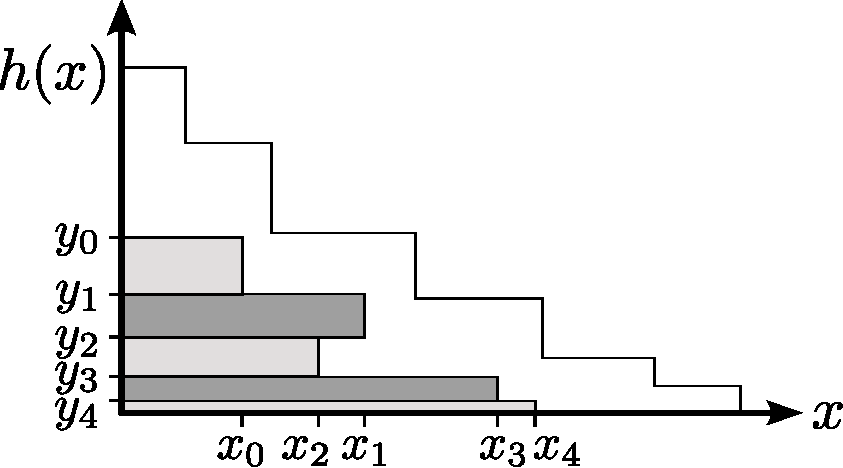
\includegraphics [width=3in]{figs/minsum} %
	\end {center}
	\caption {An illustration of the inequality
          $\int_{x=0}^{\infty} h(x) dx \ge \sum_{i \ge 0} x_i \paren { y_i - y_{i+1} }$.}
	\label {fig:proof_by_picture}
\end {figure}
%

\begin {proofof}{Theorem~\ref{thm:min-sum-set-cover}}
Let $\quota := \expctoverrlz{\rvrlz}{f(\groundset, \rvrlz)}$ be the maximum
possible expected reward, where the expectation is taken w.r.t. $\rlzprior$.
Let $\policy$ be an $\alpha$-approximate greedy policy.
Define $R_i := \quota - \avgf \paren  {\prune{\policy}{i}}$ and define $P_i := \quota - \avgf \paren  {\strictprune{\policy}{i}}$.
Let $x_i := \frac {P_i} {2 s_i}$, let $y_i := \frac {R_i} {2}$, and
let $h(x) := \quota - \avgf(\prune{\policy^*} {x})$.  
We claim $\avgf \paren
{\strictprune{\policy}{i}} \le \avgf \paren  {\prune{\policy}{i}}$ and so 
$P_i \ge R_i$.
This clearly holds if $\strictprune{\policy}{i}$ is the empty policy, and
otherwise $\policy$ can always select an item 
that contributes zero marginal benefit, namely an item 
it has already played previously.  Hence an $\alpha$-approximate greedy policy
$\policy$ can never select items with negative expected marginal
benefit, and so 
$\avgf \paren {\strictprune{\policy}{i}} \le \avgf \paren  {\prune{\policy}{i}}$. 
By Lemma~\ref {lem:greedy_rate}, $ \avgf \paren{\prune{\policy^*}
  {x_i} } \le
\avgf \paren{\strictprune{\policy} {i} } + x_i s_i$.
Therefore
\begin{equation}
  \label{eq:min-sum1}
h(x_i) \ge \quota - \avgf(\strictprune{\policy} {i}) - x_i \cdot s_i = P_i  -
\frac {P_i} {2} \ge \frac {R_i} {2} = y_i
\end{equation}

For similar reasons that $\avgf \paren {\strictprune{\policy}{i}} \le
\avgf \paren  {\prune{\policy}{i}}$, we have 
$\avgf \paren {\prune{\policy}{i-1}} \le \avgf \paren  {\prune{\policy}{i}}$, and
so the sequence $\tuple {y_1, y_2, \ldots}$  is non-increasing.
The \term monotonicity and \term submodularity of $f$ imply that $h(x)$ is
non-increasing.  Informally, this is because otherwise, if 
$\avgf(\prune{\policy^*} {x}) > \avgf(\prune{\policy^*} {x+1})$ for some
$x$, then the optimal policy must be sacrificing immediate rewards at
time $x$ in exchange for greater returns later, and it can be shown
that if such a strategy is optimal, then \term submodularity cannot hold. 
%
\eqnref{eq:min-sum1} and the monotonicity of $h$ and $i \mapsto y_i$
imply that $\int_{x=0}^{\infty} h(x)dx
\ge \sum_{i \ge 0} x_i \paren { y_i - y_{i+1} }$ (see Figure \ref
{fig:proof_by_picture}).  The left hand side is a lower bound for 
$\costminsum{\policy^*}$, and because $s_i = \alpha \paren {R_i -
  R_{i+1}}$ the right hand side simplifies to
$\frac{1}{4\alpha} \sum_{i \ge 0} P_i = \frac{1}{4\alpha}
\costminsum{\policy}$, proving $\costminsum{\policy} \le 4 \alpha \cdot \costminsum{\policy^*}$.
\end {proofof}
%

%

%

\newcommand{\gimmespace}{\phantom{$\paren{\frac{\sum }{2}}$}}


\begin{table}[p]
\subsection{A Symbol Table} \label{sec:symbols} \vspace{1em}
  \begin{tabular}{|l|p{5in}|}
\hline
$\groundset$, $\elem \in \groundset$ & Ground set of items, and an individual item. \\
\hline
$\outcomes$, $\outcome \in \outcomes$ & States an item may be in, or outcomes of selecting an item, and an individual state/outcome. \\
\hline
$\rlz$ & A realization, i.e., a function from items to states. \\
\hline
$\prlz$ & A partial realization, typically encoding the current set of observations;\\
 &  each $\prlz \subset \groundset \times \outcomes$ is a partial
 mapping from items to states. \\
\hline
$\rvrlz, \rvprlz$ & A random realization and a random partial
realization, respectively.\\
%
\hline
$\sim$ & The consistency relation: $\rlz \sim \prlz$ means $\prlz(e) = \rlz(e)$ for all $e \in \dom(\prlz)$.\\
\hline
$\rlzmasssym$ & The probability distribution on realizations.\\
\hline
$\rlzmasssym(\rlz \mid \prlz)$ & The conditional distribution on realizations: $\rlzmasssym(\rlz \mid \prlz) :=
\prob{\rvrlz = \rlz \mid \rvrlz \sim \prlz}$.\\
\hline
$\policy$ & A policy, which maps partial realizations to items. \\
\hline
$\played{\policy}{\rlz}$ & The set of all items selected by $\policy$ when run
under realization $\rlz$. \\
\hline
$\diff{\prlz}{\elem}$ & The conditional expected marginal benefit of $e$ conditioned on $\prlz$: \\
                              & $\diff{\prlz}{\elem} := \expct{f(\dom(\prlz) \cup \set{\elem}, \rvrlz) -
   f(\dom(\prlz), \rvrlz)\ | \ \rvrlz\sim\prlz}$. \\
\hline
$\diff{\prlz}{\policy}$ & The conditional expected marginal benefit of
policy $\policy$ conditioned on $\prlz$: \\
                              & $\diff{\prlz}{\policy} :=
                              \expct{f(\dom(\prlz) \cup \played{\policy}{\rvrlz}, \rvrlz) -
   f(\dom(\prlz), \rvrlz)\ | \ \rvrlz\sim\prlz}$. \\
\hline
$\substitute{\prlz}{\elem}{\outcome}$ & Shorthand for $\prlz \cup \set{(\elem, \outcome)}$.\\
\hline
$\budget$ & Budget on the cost of selected item sets.\\
\hline
$\prune{\policy}{k}$ & A truncated policy.  See Definition~\vref{def:policy-truncation} (unit costs) and Definition~\vref{def:policy-truncation-with-costs}. \\
\hline
$\strictprune{\policy}{k}$ & A strictly truncated policy.  See Definition~\vref{def:strict-prune}.\\
\hline
$\laxprune{\policy}{k}$ & A laxly truncated policy.  See Definition~\vref{def:lax-prune}.\\
\hline
$\append{\policy}{\policy'}$ & Policies $\policy$ and $\policy'$ concatenated together.  See Definition~\vref{def:policy-concatenation}.\\
\hline
$f$ & An objective function, of type $f:2^{\groundset} \times \outcomes^{\groundset} \to \NonNegativeReals$ unless stated otherwise.\\
\hline
$\avgf$ & Average benefit: $\avgf(\policy) := \expct{f(\played{\policy}{\rvrlz}, \rvrlz)}$.\\
\hline
$c$ & Item costs $c:\groundset \to \nats$.  Extended to sets via $c(S) := \sum_{e \in S} c(e)$. \\
\hline
$\acstsym$ &  Average cost of a policy: $\acst{\policy} := \expct{c(\played{\policy}{\rvrlz})}$.\\
\hline
$\awstsym$ &  Worst-case cost of a policy: $\wcst{\policy} := \max_{\rlz}{c(\played{\policy}{\rlz})}$.\\
\hline
$\costminsumsym$ &  Min-sum cost of a policy: $\costminsum{\policy} := \sum_{t =  0}^{\infty} \paren{\expct{f(\groundset, \rvrlz)} -
      \avgf(\strictprune{\policy}{t})}.$ \\
\hline
$\condcost{\prlz}{\policy}$ & Conditional average policy cost:
$\condcost{\prlz}{\policy} :=
\expct{c(\played{\policy}{\rvrlz})  \mid  \rvrlz \sim  \prlz}$. \ignore{\gimmespace} \\
\hline
$\alpha$ & Approximation factor for greedy optimization in an $\alpha$-approximate greedy policy.\\
\hline
$\quota$ & Benefit quota.  Often $\quota = \expct{f(\groundset, \rvrlz)}$.\\
\hline
$\eta$ & Coverage gap: $\eta = \sup \set{ \eta'  :  f(S, \rlz) > Q
  - \eta' \text{ implies }f(S, \rlz) \ge Q \text{ for all }S, \rlz }$.\\
\hline
$\indicator{P}$ & The indicator for proposition $P$, which equals one if $P$ is true and
zero if $P$ is false.\\
\hline    
\end{tabular}
 \caption{Important symbols and notations used in this article}  \label{table:symbol-table}
\end{table}

%

%
%
%
%

%

\subsection{Proof of Approximation Hardness in the Absence of \Term
  Submodularity}  \label{sec:proof-approx-hardness}

We now provide the proof of \thmref{thm:hardness} whose statement 
appears on page~\pageref{thm:hardness} in~\secref{sec:hardness}.\\


%
\begin{proofof}{\thmref{thm:hardness}}
%
%
%
%
%
%
%
%
%
%
%
%
%
%
%
%
%
%
%
%
%
%
We construct a hard instance based on the following
intuition.  We make the algorithm go ``treasure hunting''.  There is a
set of $\ntreasure$ locations $\set{0, 1,, \ldots, \ntreasure-1}$, there is a treasure
at one of these locations, and the algorithm gets unit reward if it
finds it, and zero reward otherwise.  There are $\nmaps$ ``maps,''
each consisting of a cluster of $\mapsize$ bits, and each
purporting to indicate where the treasure is, and each map is stored
in a (weak) secret-sharing way, so that querying few bits of a map
reveals nothing about where it says the treasure is.
Moreover, all but one of the maps are \emph{fake}, and there is a 
puzzle indicating which map is the correct one
indicating the treasure's location.  Formally, a fake map is one
which is probabilistically independent of the location of the treasure,
conditioned on the puzzle.


Our instance will have three types of items, $\groundset =
  \groundset_T \uplus \groundset_M \uplus \groundset_{P}$, where
  $|\groundset_{T}|=\ntreasure$ encodes where the treasure is,
  $|\groundset_{M}|=\nmaps \mapsize$ encodes the maps, and
  $|\groundset_{P}|=\nmatrix^{3}$ encodes the puzzle, where 
 $\nmaps,\ntreasure,\mapsize$ and $\nmatrix$ are specified below.
  All outcomes are binary, so that $\outcomes=\{0,1\}$, and we
  identify items with bit indices.  Accordingly we say that 
  $\rlz(\elem)$ is the value of bit $\elem$.
  For all $e\in
  \groundset_{M}\cup\groundset_{P}$, $\prob{\rvrlz(e)=1}=.5$
  independently. The conditional distribution of 
  $\rvrlz(\groundset_{T})$ given $\rvrlz(\groundset_{M}\cup\groundset_{P})$
  will be deterministic as specified below. Our objective function $f$
  is linear, and defined as follows:
$$f(\groundsubset,\rlz)=|\{e\in \groundsubset\cap\groundset_{T}:\rlz(e)=1\}|.$$


\noindent We now describe the puzzle, which is to compute 
$i(P) := (\perm(P) \mod p) \mod 2^\ell$ for a suitable random matrix $P$,
and suitable prime $p$ and integer $\ell$, where 
$\perm(P) = \sum_{\sigma \in S_{\nmatrix}} \prod_{i=1}^n P_{i\sigma(i)}$ is the permanent of $P$.
We exploit Theorem~$1.9$ 
of~\citet{FeigeL97} in which they show that if there exist constants
$\eta, \delta > 0$ such that a randomized polynomial time algorithm can
compute $(\perm(P) \mod p) \mod 2^\ell$ correctly with probability 
$2^{-\ell}(1 + 1/\nmatrix^\eta)$, where $P$ is drawn uniformly at random from 
$\set{0,1,2, \ldots, p-1}^{\nmatrix \times \nmatrix}$, $p$ is any prime
superpolynomial in $\nmatrix$, and $\ell \le p\paren{\frac{1}{2} - \delta}$,
then $\class{PH} = \class{AM} = \Sigma^P_2$.
%
To encode the puzzle, 
%
%
%
we fix a prime $p \in [2^{\nmatrix-2}, 2^{\nmatrix-1}]$ and use the $\nmatrix^3$ bits of
$\rlz(\groundset_P)$ to sample $P = P(\rlz)$ (nearly) uniformly at random from 
$\set{0,1,2, \ldots, p-1}^{\nmatrix \times \nmatrix}$ as follows.
For a matrix $P \in \integers^{\nmatrix \times \nmatrix}$, we let $\numberof(P) := \sum_{ij}P_{ij}\cdot
p^{(i-1)\nmatrix+(j-1)}$ define a base $p$ representation of $P$.
Note $\numberof(\cdot)$ is one-to-one for $\nmatrix \times \nmatrix$ matrices with entries in
$\integers_{p}$, so we can define its inverse 
$\invnumberof(\cdot)$.
The encoding $P(\rlz)$ interprets the bits $\rlz(\groundset_{P})$ as
an integer $x$ in $[2^{\nmatrix^3}]$, and computes $y = x \mod (p^{\nmatrix^2})$.
If $x \le \floor{2^{\nmatrix^3}/p^{\nmatrix^2}} p^{\nmatrix^2}$, then $P =
\invnumberof(y)$.
Otherwise, $P$ is the all zero matrix.
This latter event occurs with probability at most $p^{\nmatrix^2}/2^{\nmatrix^3} \le
2^{-\nmatrix^2}$, and in this case we simply suppose the 
algorithm under consideration finds the treasure and so gets unit reward.
This adds $2^{-\nmatrix^2}$ to its expected reward.
So let us assume from now on that $P$ is drawn uniformly at random.


Next we consider the maps.  
Partition $\groundset_{M}=\biguplus_{i=1}^{\nmaps}M_{i}$ into $\nmaps$
maps $M_{i}$, each consisting of $\mapsize$ items.
For each map $M_{i}$, partition
its items into $\mapsize/\log_{2} \ntreasure$ groups of $\log_{2}
\ntreasure$ bits each, so that the bits of each group encode a 
$\log_{2} \ntreasure$ bit binary string.
Let $v_{i} \in \set{0,1,\ldots,\ntreasure-1}$ be the XOR of these $\mapsize/\log_{2} \ntreasure$
binary strings, interpreted as an integer (using any fixed encoding). 
We say
$M_{i}$ \emph{points to} $v_{i}$ as the location of the treasure.
A priori, each $v_{i}$ is uniformly distributed in $\{0,...,\ntreasure-1\}$. For a
particular realization of $\rlz(\groundset_{P}\cup\groundset_{M})$,
define $v(\rlz) := v_{i(P(\rlz))}$.  We set $v(\rlz)$ to be the location of the
treasure under realization $\rlz$, i.e., we label $E_{T} = \set{e_0,e_1,\ldots, e_{\ntreasure-1}}$ and ensure 
$\rlz(e_{j}) = 1$ if $j = v_{i(P(\rlz))}$, and $\rlz(e) = 0$ for
all other $e \in E_{T}$.
%
Note the random variable $v = v(\rlz)$ is distributed
uniformly at random in $\{0,1,\dots,\ntreasure-1\}$.  Note that this still holds
if we condition on the realizations of any set of $\mapsize/\log_{2} \ntreasure - 1$
items in a map, because in this case there is still at least one group
whose bits remain completely unobserved.


Now consider the optimal policy with a budget of $k=\nmatrix^{3}+\mapsize+1$ items to pick.
Clearly, its reward can be at most $1$.  However, given a budget of $k$, 
a computationally unconstrained policy can exhaustively sample
$\groundset_{P}$, solve the puzzle (i.e., compute $i(P)$), read the
correct map (i.e., exhaustively sample $M_{i(P)}$), decode the map
(i.e., compute $v=v_{i(P)}$), and get the treasure (i.e., pick
$e_{v}$) thereby obtaining a reward of one. 


Now we give an upper bound on the expected reward $R$ of any randomized
polynomial time algorithm $\Alg$ with a budget of $\beta k$ items, 
assuming $\Sigma^P_2 \neq
\class{PH}$. 
Fix a small constant $\gamma > 0$, and set $\mapsize = \nmatrix^3$ and $\nmaps = \ntreasure = \nmatrix^{1/\gamma}$.
%
%
%
%
We suppose we give $\Alg$ the realizations $\rlz(\groundset_M)$ for free.
We also replace its budget of $\beta k$ items with a 
budget of $\beta k$ specifically for map items in $E_{M}$ and
an additional budget of $\beta k$ specifically for the treasure locations in
$E_{T}$. 
Obviously, this can only help it. 
As noted, if it selects less than 
$\mapsize/\log_{2} \ntreasure$ bits from the map $M_{i(P)}$ indicated by $P$, the
distribution over $v_{i(P)}$
conditioned on those realizations is still uniform.  Of course,
knowledge of $v_{i}$ for $i \neq i(P)$ is useless for getting reward.
Hence $\Alg$ can try at most 
$\beta k \log_{2}(\ntreasure) / \mapsize = o(\beta k)$ 
%
%
%
maps in an attempt to find $M_{i(P)}$.
Note that if we have a randomized algorithm which given a random $P$ drawn from 
$\set{0,1,2,  \ldots, p-1}^{\nmatrix \times \nmatrix}$ always outputs a set $S$ of
integers of size $\alpha$ such that $\prob{i(P) \in S} \ge q$, then we can use it to
construct a randomized algorithm that, given $P$, outputs an integer $x$ such
that $\prob{i(P) = x} \ge q/\alpha$, simply by running the first algorithm
and then selecting a random item of $S$.
If $\Alg$ does not find $M_{i(P)}$, the distribution on the treasure's location
is uniform given its knowledge.  Hence it's budget of
$\beta k$ treasure locations can only earn it expected reward at most $\beta k/\ntreasure$.
Armed with these observations and 
Theorem~$1.9$ in the work of~\citet{FeigeL97} and our complexity theoretic
assumptions, we infer
%
$\expct{R} \le o(\beta k) \cdot  2^{-\ell}(1 + 1/\nmatrix^{\eta}) +
\beta k/\ntreasure + 2^{-\nmatrix^2}$.
Since $\mapsize = \nmatrix^3$ and $\nmaps = \ntreasure = \nmatrix^{1/\gamma}$ and $\gamma = \Theta(1)$
and $\eta = 1$ and $\ell = \log_{2} \nmaps$ and $k = \nmatrix^3 +
\mapsize + 1 = 2 \nmatrix^3 + 1$,
we have 
$$\expct{R} \le \frac{\beta k}{\ntreasure}\paren{1 + o(1)} = 
2\beta\nmatrix^{3 - 1/\gamma}(1 + o(1))\mbox{.}$$


%
%
\noindent Next note that $|\groundset|=\ntreasure+\nmaps \mapsize
+\nmatrix^{3} =  \nmatrix^{3+1/\gamma}(1 + o(1))$.
Straightforward algebra shows that in order to ensure
$\expct{R}=o( \beta/|\groundset|^{1-\varepsilon})$, 
it suffices to choose $\gamma \le \varepsilon/6$. Thus, under our
complexity theoretic assumptions, any polynomial time randomized
algorithm $\Alg$ with budget $\beta k$ achieves at most
$o(\beta / |\groundset|^{1-\varepsilon})$ of the value obtained by the
optimal policy with budget $k$, so the approximation ratio is $\omega(|\groundset|^{1-\varepsilon}/\beta)$.
\end{proofof}


%
%
%
%
